\documentclass[conf]{new-aiaa}
%\documentclass[journal]{new-aiaa} for journal papers
\usepackage[utf8]{inputenc}

\usepackage{graphicx}
\usepackage{amsmath}
\usepackage{gensymb}
\usepackage{biblatex}
\usepackage[version=4]{mhchem}
\usepackage{siunitx}
\usepackage{longtable,tabularx}
\setlength\LTleft{0pt} 
\addbibresource{sources.bib}


\title{Structural and Material Analysis of the SR-71 Blackbird}

\author{Wyatt O. Welch\footnote{Viasat Satellite Controller, AE 310 Structures, wwelch0753@sdsu.edu.}}
\affil{SDSU Aerospace Engineering Student, enrolled in AE 310, San Diego, CA, 92115}


\begin{document}

\maketitle

\begin{abstract}
The purpose of this paper is to provide background, structural analysis, and material component analysis of Lockheed Martin's SR-71 Blackbird, developed and first flown in 1964, and retired in 1990. The goal is to inform readers of the fascinating development and structure that went into making the SR-71 such a unique jet.
\end{abstract}

\section{Introduction}
\lettrine{T}{his} document is intended to cover the materials used in the development of the SR-71, as well as detail at least one aspect of the structure that is interesting and worth pointing out for the readers' edification.

The formatting of this paper will first cover the history of the SR-71 from a distance, and describe the interesting necessities the Skunk Works team had to follow in order to create such a unique and stylish jet. From the history, the author will single out a single aspect of the structure and describe in detail the uses, reasons for its existence, and any future applications similar structures have had on other planes. The final section will cover the materials used in the body, and interior of the SR-71 with an Aerospace lens. Why were these materials chosen over others? What was required leading up to the use of these materials? etc. With these questions being answered, the goal is for the reader to have a better understanding of the context, and the details of what makes the SR-71 the SR-71.

\section{History and Background}
The Skunk Works division was formed in 1943 in response to Germany's Me-262 fighter jet with the sole purpose of pushing America's aeronautics back into the forefront with the first US jet. Within 143 days, beating their set deadline, Skunk Works had the P-80 Shooting Star, which went on to win the first jet-vs-jet dogfight in 1950. 
With this beginning, Skunk Works was commissioned to create an elusive spy plane, one that could outrun missiles and avoid satellite detection. On July 3, 1963, the team had done just that with the SR-71. With heat-dissipating black paint, and an incredible top speed of Mach 3.3, this remains the fastest air-breathing manned aircraft in the world \cite{skunkStory}.\par
The basis of the SR-71 was formed from the A-12, which was an aluminum jet that was able to reach great speeds, but had an Achilles' heel in the aluminum airframe. This material was unable to withstand the over 900$^{\circ}$F caused by the air friction on the body. With aluminum out of the question, titanium was the best choice in order to deal with the heat. The major supplier for titanium at the time of the Cold War was the USSR. With the ingenuity befitting the Skunk Works team, the US was able to secure the needed titanium from the Russians through the use of third world countries, shell corporations, and fake operations (such as a factory needing the titanium for pizza ovens) \cite{pizzaSource}.\par
The manufacturing process for titanium was a massive challenge by itself. With the standard for creating pure and reliable titanium having been invented only a few years before, many new tools and methods would need to be created in order to work on such an intricate creation as the Blackbird. Throughout the manufacturing process, there were issues that the team ran into. One year, they noticed welded parts would fail early in the summer, but would last far longer when welded that winter. The issue was tracked to chlorine the Burbank Water Treatment Plant added to fight algae, and from then on distilled water was used to clean welded parts. \par
Inventions were also needed to get this project to be as efficient and sustainable as possible. Drilling holes started as a very grueling and wasteful process, since drill bits used to make holes for rivets would break in on average 17 holes. Through necessary innovation, new techniques and technology allowed for over 100 uses \cite{Titanium}.\par
When in the air, the surface of the plane would easily pass 900$^{\circ}$F, which would mean the interior would also become extremely hot. It was discovered that the fuel itself could be heated to upwards of 190$^{\circ}$F and would have a high risk of lighting. Due to this, it was required to create a fuel with an extremely high flash point. It was said to have been so high that crewmen could throw lit matches into the fuel and it would be put out. With all of these advancements and hoops that were required to jump through, it is no wonder that the SR-71 is world famous for the brilliant engineering that went into it.
\pagebreak

\begin{figure}
    \centering
    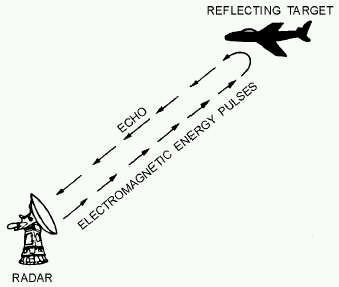
\includegraphics[width=0.5\linewidth]{image1.png}
    \caption{Radar Pinging Target}
    \label{fig1}
\end{figure}

\section{Special Structures}
For many, the first look upon the SR-71 gives the impression of a particularly organically shaped jet. The curving of the body with a slope off that ends a seemingly sharp leading edge seems purely stylish by most standards. However, there is actually a key use to this sloping design that gives another reason why the SR-71 is and was so dominant in nearly everything it does. A reminder from the history, the two requirements the USAF gave to Skunk Works were speed, and stealth. We have already looked at the speed, and consequences of the speed, so now we must go to stealth. While nothing is fully protected from radar, stealth is used to minimize the chance, or time it takes, for the jet to be recognized by enemies on the ground using radar or satellites.\par
Shown in \ref{fig1} is a layman's example of how radar identifies aircraft. To avoid being detected, the SR-71 employs the oddly shaped body and wings, which act to redirect the majority of echo back to the radar. You can think of this as an angled mirror reflecting a sunbeam, only it redirects in thousands of different directions. While some signals will make their way back to the ground site, with that much of a diminished return signal, computers and humans monitoring were likely to interpret the signals as interference from uncontrollable variables like birds \cite{airframe}.\par
For satellites, the technique to evade detection is even more simple, however implementation makes it a far more difficult task to pull off. In the same way your camera cannot focus on both the foreground and the background, satellites cannot focus on low altitude and high altitude planes. At the time the SR-71 was in use, it was unreasonable to take a satellite's entire functionality only for the off chance of catching this rare and elusive plane. In addition, for both radar and satellites, the speed of the SR-71 made all detection both nearly impossible and nearly pointless, because by the time you identified the ship, and got enough readings to calculate trajectory and speed, it was likely to already be out of your airspace. Mach 3.3 is nothing to scoff at, and it made any retaliation near fruitless.

\section{Material Analysis}
There certainly is much to be said about the unique materials that went into the SR-71. With all the talk of titanium, it is important to establish the importance of titanium as the choice for this project. Truly no other metal or alloy would have sufficed. While titanium does not have better strength than steel, weighs heavier than aluminum, and even a worse temperature tolerance than steel, the combination of the average results made for the overall better pick. It is as the saying goes; \textit{"A jack of all trades is a master of none, but will always be better than a master of one"}. With that acknowledgment we can consult any handy guide to choosing materials to determine what choice best fits the requirements of the SR-71 (high heat tolerance, strong, dense, not too heavy).\par
As observable in \ref{fig2}, titanium holds one of the highest strengths depending on the alloy, but holds a far lower density than that of steel. If this were also to be considered with melting temperatures, it remains little wonder why this was the chosen material to make up \%92 of the ship "inside and out" \cite{BBC}. The reason this remarkable metal is not seen on all planes is due to the expenses. Despite titanium being the ninth most common element in earths crust, even surpassing carbon, it is still incredibly difficult to purify and work with, making it unreasonable for large projects \cite{Titanium}. \par
Beyond the titanium, the paint used to coat the exterior of the ship was also a technically useful material. The paint had special properties that absorbed and emitted heat throughout the ship, supporting the many other cooling systems on board, and the paint also helped both with reflecting radar as well as disguising the ship during night operations.\par
Just to show how much attention to detail was given to every aspect of the SR-71, it is worth discussing the tires. In order to deal with the fuselage reaching temperatures upwards of 900$^{\circ}$, tires would need to be made in such a way as to not let them melt during flights. As a result, BF Goodrich developed a rubber compound with aluminum powder to keep the tires from melting away. In addition, the tires were filled with nitrogen, since it is stable, suppresses fires, does not expand in heat, and does not absorb water vapor. These issues were unheard of before the development of the SR-71, and is a sign of the push this craft had on the industry \cite{boom}.

\begin{figure}
    \centering
    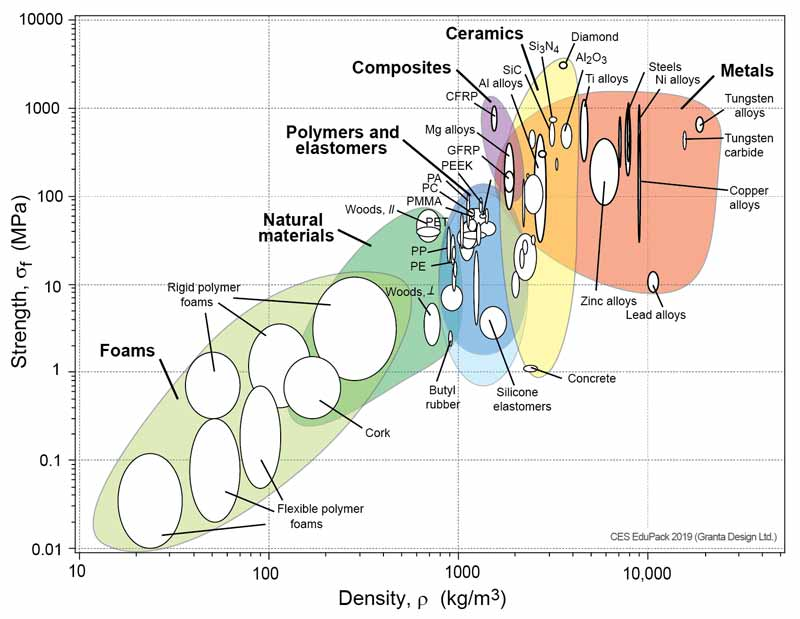
\includegraphics[width=.75\linewidth]{image2.png}
    \caption{Strength vs. Density of Common Materials}
    \label{fig2}
\end{figure}

%paint
%wheels
%titanium (image)

\section{Conclusion}
The work required to make any jet fly is something few could claim to have the ability to do, however the brilliant minds that created the SR-71 stand in a class of their own. With a complex history leading to an extremely taxing request, and the thousands of obstacles in the way of each task, it is a world-wide wonder how this jet could have been created with the resources, and knowledge known at the time. In such a complex and ever-changing field, it boggles the mind how the SR-71 could still be the record holder for three separate world records, and have been holding them since the 1960's. The structure's fascinating and unique design allows for the craft to have extremely capable uses as a spy jet, and the materials used in every single piece of this craft make it a compilation of mankind's genius. The SR-71 Blackbird truly is a work of art.

\newpage
\printbibliography[]
\end{document}
